\chapter{Programas de Física para o Ensino Médio}
\thispagestyle{empty}
\label{cap: prgFisica}
O acesso ao Planejamento Anual do Professor Supervisor não foi viabilizado neste estágio, de modo que a análise que aqui se estende, tem por base os materiais disponibilizados às turmas de segundo e terceiro ano, no ambiente virtual \emph{Google Classroom}. Nesta análise, não se inclui os primeiros anos em virtude de que o Professor Supervisor não as atendia no momento em que foi escrito este relatório.

\section{Conteúdos Abordados nos Segundos Anos}
A \autoref{fig:classroomSegundoAno} mostra os últimos conteúdos de Física do segundo ano lecionados até o mês de setembro do ano de 2022. Nela podemos ver uma estrutura de tópicos inseridos à medida que o professor vai avançando na disciplina.
\vspace{.5cm} 
\begin{figure}[!htpb]
    \begin{center}
        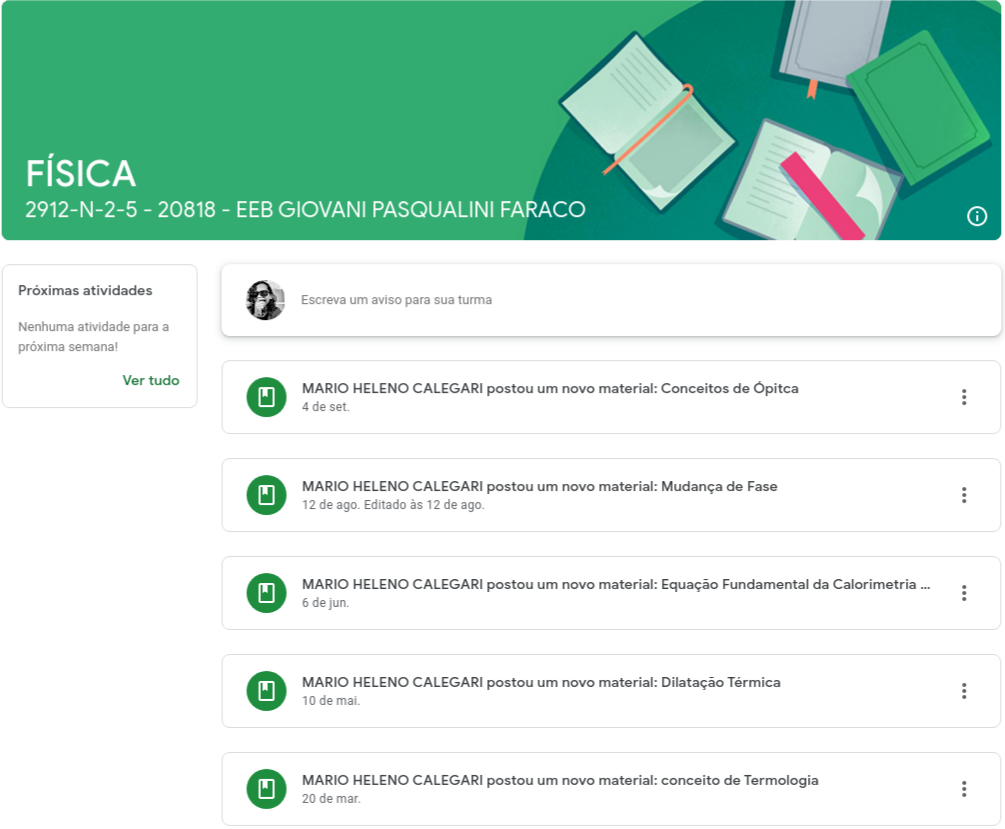
\includegraphics[width=.95\textwidth]{03-elementos/03.2_textual/03.2.1_fig/programaFisica2-5.png}
        \caption{Conteúdos de Física 2°(5) -- Google Classroom}
        \label{fig:classroomSegundoAno}
    \end{center}    
\end{figure}

Esta unidade trata essencialmente dos assuntos relacionados à Energia. A sequência completa até o momento é apresentada como segue: \emph{1. Energia Mecânica, 2. Termologia, 3. Dilatação Térmica, 4. Equação Fundamental da Calorimetria, 5. Mudança de Fase e 6. Conceitos de Óptica.}

Assim disposto, vemos que a sequência segue ainda a forma apresentada tradicionalmente nos livros didáticos da disciplina, com exceção do tópico Energia Mecânica, o qual normalmente é tratado ao final do primeiro ano do Ensino Médio. As seções internas de cada tópico apresentado no Google Classrom segue a seguinte abordagem: apresentação dos conceitos/teorias, seguido de alguns exemplos de substituição direta e finalizando com uma lista de exercícios. Para melhor compreensão e visualização, um elemento da unidade relacionada a Dilatação Térmica dos materiais pode ser visto na íntegra na \autoref{anx:materialAnexoDilatacaoTermica} do Anexo \ref{anx:materiaisAnexo}.  

Uma das características mais marcantes da \ac{BNCC}, diz respeito à \emph{flexibilização dos currículos}. O atendimento a este princípio exige que \emph{``[\ldots] se rompa com a centralidade das disciplinas, em prol de um currículo que contemple a complexidade das relações existentes entre os ramos da ciência''} \cite{BRASIL:2017}. Além disso, deve-se estimular continuamente o protagonismo dos estudantes, de forma que

\begin{citacao}
    ``evidencie a contextualização, a diversificação e a transdisciplinaridade ou outras formas de interação e articulação entre diferentes campos de saberes específicos, contemplando vivências práticas e vinculando a educação escolar ao mundo do trabalho e à prática social e possibilitando o aproveitamento de estudos e o reconhecimento de saberes adquiridos nas experiências pessoais, sociais e do trabalho.'' \cite{BRASIL:2018}
\end{citacao}
Neste sentido entende-se que não só a predisposição, como até mesmo os próprios assuntos ofertados, ao atender aos pressupostos da Base, devam ser capazes de promover um diálogo constante com as realidades locais de cada unidade escolar. Da forma como é estabelecida, estas exigências não privilegiam uma sequência em detrimento da outra, apenas atentam sobre as particularidades a que cada contexto e/ou grupo escolar esteja imerso em sua realidade de ensino, desde que possibilite o protagonismo dos estudantes, de modo a proporcionar o pensamento crítico perante as questões da contemporaneidade.

Já a \ac{PCSC} trata o tema Energia como objeto de estudo designado por meio de \emph{conceitos fundantes}, orienta que o ensino de Física deva seguir de forma contextualizada e centrada nestes conceitos de forma dialogada e estimulante \cite[p.~164]{BRASIL:2017}. Estas duas visões não encontram-se dissonantes, mas reforçam-se na concepção de um currículo interdisciplinar, estimulante, contextualizado e dialógico.

Considerando o exposto, vê-se ainda certa resistência à adequação deste currículo, em atenção às novas exigências propostas pelas reformas, ao menos no que tange o planejamento de um currículo contextualizado, dialógico e próximo à realidade do estudante.

\section{Conteúdos Abordados nos Terceiro Anos}
Seguindo como na seção anterior, tem-se na \autoref{fig:classroomTerceiroAno} a sequência utilizada até o momento, contendo a estrutura dos últimos tópicos das aulas ministradas entre as turmas de terceiro ano.
\vspace{.5cm} 
\begin{figure}[!ht]
    \begin{center}
        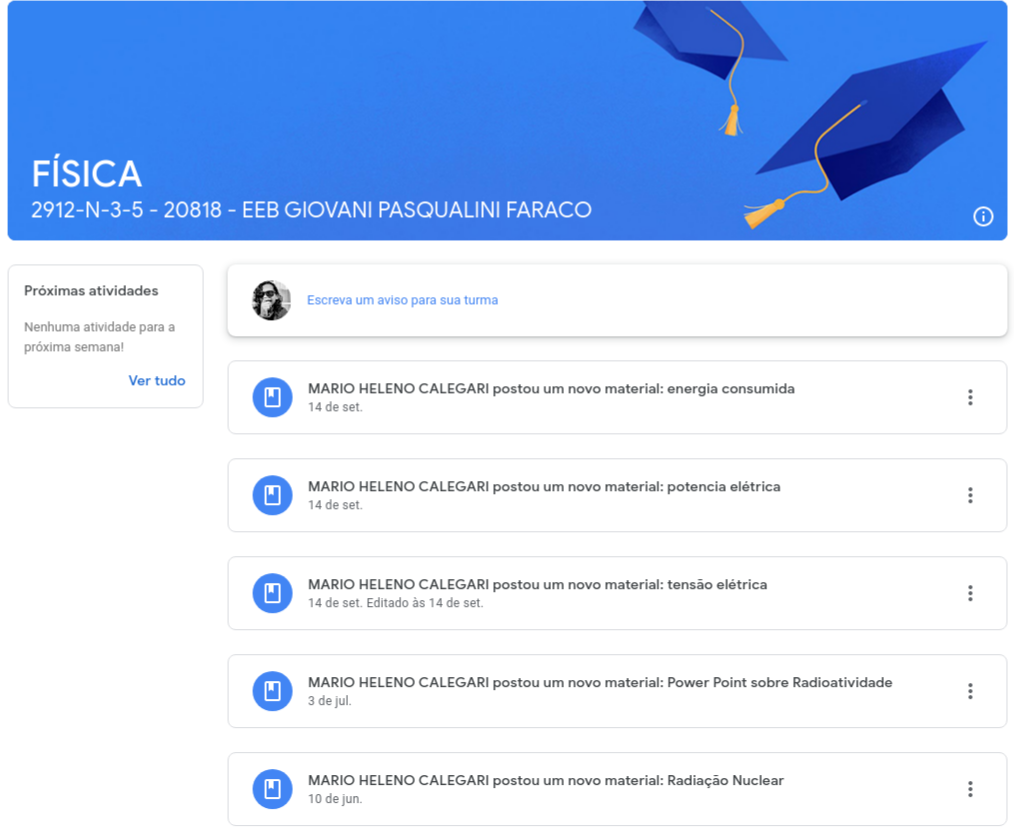
\includegraphics[width=\textwidth]{03-elementos/03.2_textual/03.2.1_fig/programaFisica3-5.png}
        \caption{Conteúdos de Física 3°(5) -- Google Classroom}
        \label{fig:classroomTerceiroAno}
    \end{center}    
\end{figure}

Aqui vemos uma abordagem similar a anterior, seguindo a ordem dos livros didáticos tradicionais: \emph{1. Conceitos de Eletricidade, 2. Lei de Coulomb, 3. Corrente Elétrica, 4. Radiação Nuclear, 5. Radioatividade, 6. Tensão Elétrica, 7. Potência Elétrica e 8. Energia Consumida}. A inserção dos tópicos relacionados à \emph{Radiação e Radioatividade} quebra a estrutura tradicional dos livros, uma vez que este assunto é visto (quando visto), em tópicos mais avançados, junto com ondas eletromagnéticas e/ou estrutura da matéria.

A metodologia utilizada, mais especificamente no tópico relacionado à Radioatividade, aborda o assunto do ponto de vista da História da Ciência -- \emph{História da Radiação}, precisamente. A abordagem desdobra-se, dentre outras formas, trazendo o contexto das descobertas científicas da época para dentro da sala de aula, atendendo a algumas das exigências da \ac{PCSC} como, por exemplo:

\begin{citacao}
    ``O aprofundamento na formação científica envolve a caracterização dos elementos químicos partindo de suas propriedades, seguindo-se de sua representação e modelagem, \ldots enfocando a evolução dos modelos atômicos, incluindo modelos quânticos que permitem a compreensão da tabela periódica dos elementos. Ao mesmo tempo, se reconhece e apresenta a ciência como uma construção humana, associada ao desenvolvimento produtivo, buscando assim enfatizar a presença das tecnologias em todos os períodos da história econômica e em todos os setores da vida.'' \opcit[p.~169--170]{PCSC:2014}
\end{citacao}
Sendo assim, configura-se aqui uma tímida aproximação deste currículo com a Proposta de Santa Catarina, capaz de contribuir para a formação do pensamento crítico e autonomia de pensamento, por meio da reflexão à cerca do desenvolvimento da ciência como atividade humana sujeita aos paradigmas de sua época.